%%%% Weekly Report Information %%%%
\newcommand{\handoutName}{Weekly report}
\newcommand{\handoutdate}{\today}
%\newcommand{\duedate}{}
% Header template used for Weekly Reports
\documentclass[11pt,twoside]{article}

\setlength{\oddsidemargin}{0pt}
\setlength{\evensidemargin}{0pt}
\setlength{\textwidth}{6.5in}
\setlength{\topmargin}{0in}
\setlength{\textheight}{8.5in}
\setlength{\voffset}{0in}

\providecommand{\titlesize}{small}


\usepackage{graphicx}
%\usepackage{subfigure}
\usepackage{palatino}
%\usepackage{cmbright}
\newcommand{\myMargin}{1.00in}
%\usepackage[pdftex]{hyperref}
\usepackage[small,bf]{caption}
%\usepackage{amsmath}
\usepackage[usenames,dvipsnames]{color}
\usepackage{fancyhdr}
\pagestyle{fancy}
\usepackage{datetime}
\usepackage{fancyvrb}
\usepackage{color}
\usepackage[\titlesize, compact]{titlesec}
\usepackage{multicol}
\usepackage{enumitem}
\usepackage{pdfpages}
\usepackage{mdwlist}
\usepackage{caption}
\usepackage{subcaption}
\usepackage{hyperref}
\usepackage[cmex10]{amsmath}
\usepackage{algorithmicx}
\usepackage[ruled]{algorithm}
\usepackage{algpseudocode}
\renewcommand\labelenumi{\textbf{\theenumi) }}
\newcommand\algorithmicinput{\textbf{Input:}}
%\newcommand\INPUT{\item[\algorithmicinput]}
\newcommand\algorithmicassume{\textbf{Assume:}}
%\newcommand\ASSUME{\item[\algorithmicassume]}

\newdateformat{dashdate}{\THEYEAR-\twodigit{\THEMONTH}-\twodigit{\THEDAY}}
\def\Tiny{\fontsize{3pt}{3pt}\selectfont}

\providecommand{\handoutName}{Handout title}
\providecommand{\handoutdate}{Handout date}
\providecommand{\duedate}{}

\lhead{Meeting with Prof. Becker\\
Spring, 2017}
\chead{}
\rhead{ Shiva Shahrokhi\\
\handoutdate }
\lfoot{}
\cfoot{\thepage}
\rfoot{\dashdate \Tiny \textcolor{Gray}{\today}}
\renewcommand{\headrulewidth}{0.4pt}
\renewcommand{\footrulewidth}{0.4pt}

\begin{document}

\vspace{0.60in}
\begin{center}
{\Large\textbf{\handoutName}}\\
\vspace{0.03in}
\textbf{\duedate}\\
\end{center}

\newcommand{\todo}[1]{
  \textcolor{Red}{
    \begin{tabular}{|c|}
      \hline
      \em \large \bfseries todo: \normalfont \normalsize #1 \\
      \hline
    \end{tabular}}
}


\section{My \emph{Objectives} this week: Optimal Solution for the algorithm for two robots positioning using friction}
\begin{itemize}
\item make sure three move works for all cases
\item make the rotations work correctly
\item complete the algorithm so that it also considers the not achievable sets.
\end{itemize}



\section{My \emph{Accomplishments} this week}


\begin{itemize}
\item All the rotations and three moves work.
\item Not achievable part also works.
\item The paper is now drafted and all the covariance stuff is out. (Github is updated)
\item I made these two images:
\end{itemize}

\begin{figure}[h]
\begin{center}
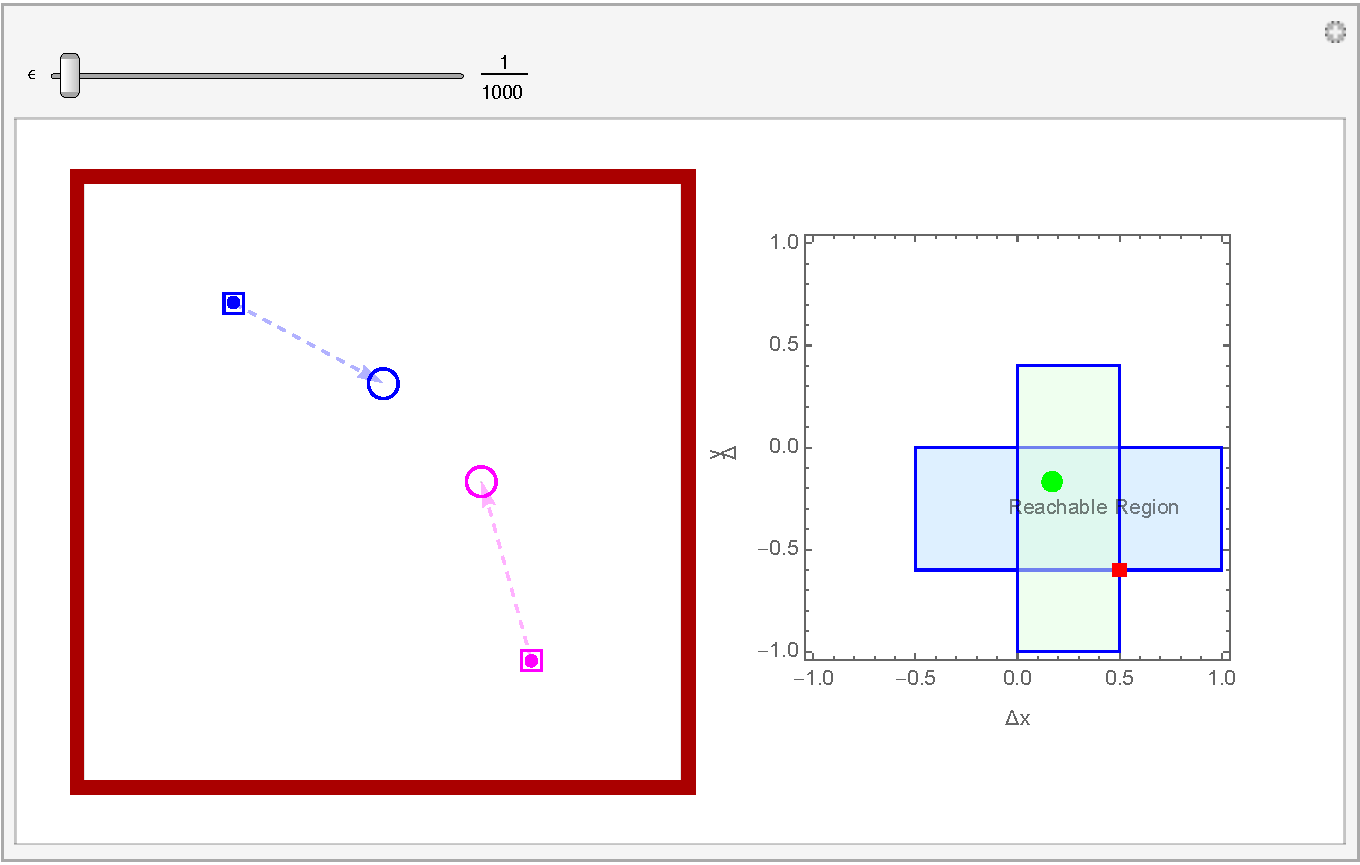
\includegraphics[width=10cm]{ReachableRegion1move.pdf}
\caption{The two rectangles shows the reachable sets of the robots.}
\end{center}
\end{figure}
\begin{figure}[h]
\begin{center}
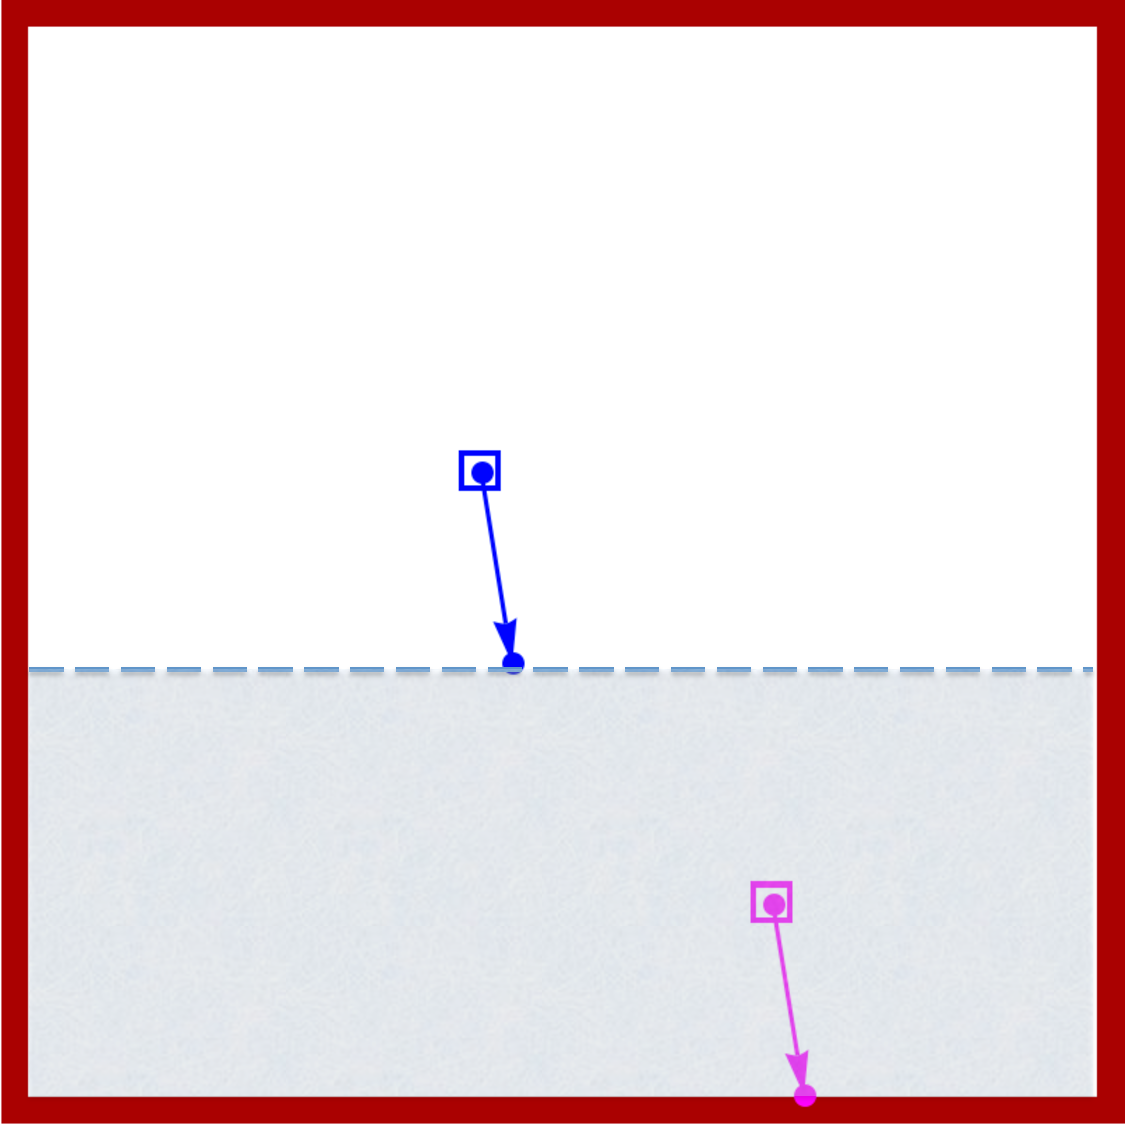
\includegraphics[width=10cm]{twoRobotRegion.pdf}
\caption{The area where the not touching robot can get in one move to adjust $\Delta gx$ and $\Delta gy$.}
\end{center}
\end{figure}
\section{My \emph{Plan} for next week}

\begin{itemize}
\item Complete debugging the optimal function A star algorithm.
\item Rewrite the whole paper with the new algorithm.
\end{itemize}

\subsection{Meeting with Dr. Becker  }

\begin{itemize}
\item Nothing to mention. I will give my progress report in my next meeting. 
\end{itemize}

\end{document}
